\section{Desenvolvimento}
\label{sec:desenvolvimento}

Esta seção descreve o protótipo experimental: como foi implementado, com quais parâmetros, quais algoritmos executa, quais scripts automatizam o processo, quais cenários foram avaliados e em que ordem tudo roda. Todo o código está no repositório do projeto (\linkProjeto).

\subsection{Implementação realizada}

O protótipo é um pacote Python organizado em módulos com responsabilidades separadas (Figura~\ref{fig:arquitetura}). A separação garante que o único componente que muda entre FedAvg e FedProx seja a função de perda local, e não o restante do \textit{pipeline}.

\begin{figure}[ht]
    \centering
    \begin{tikzpicture}[
        font=\scriptsize,
        mod/.style={draw, rounded corners=2pt, fill=azul!6, minimum width=2.45cm, minimum height=0.62cm, align=center},
        cli/.style={draw, rounded corners=2pt, fill=gray!10, minimum width=2.45cm, minimum height=0.62cm, align=center},
        arr/.style={-{Stealth[length=4pt]}, thick},
        node distance=0.38cm and 0.3cm
    ]
        \node[cli] (grid) {\texttt{grid.py}\\ gera configurações};
        \node[cli, right=of grid] (run) {\texttt{run.py}\\ executa 1 configuração};
        \node[mod, below=of grid] (data) {\texttt{data.py}\\ partições};
        \node[mod, below=of run] (strat) {\texttt{strategies.py}\\ servidor};
        \node[mod, below=of data] (client) {\texttt{client.py}\\ treino local};
        \node[mod, below=of strat] (models) {\texttt{models.py}\\ CNNs};
        \node[mod, below=of client] (metrics) {\texttt{metrics.py}\\ tempo, acurácia};
        \node[cli, below=of models] (csv) {\texttt{results/*.csv}};
        \node[cli, below=0.38cm of metrics] (bench) {\texttt{microbench.py}\\ custo em CPU};
        \node[cli, below=0.38cm of csv] (ana) {\texttt{analysis.py}\\ figuras e testes};
        \draw[arr] (grid) -- (run);
        \draw[arr] (run) -- (strat);
        \draw[arr] (run.south west) -- (data.north east);
        \draw[arr] (strat) -- (client);
        \draw[arr] (data) -- (client);
        \draw[arr] (client) -- (models);
        \draw[arr] (client) -- (metrics);
        \draw[arr] (metrics) -- (csv);
        \draw[arr] (bench) -- (ana);
        \draw[arr] (csv) -- (ana);
    \end{tikzpicture}
    \caption{Módulos do protótipo e suas dependências. Em cinza, os pontos de entrada e saídas; em azul, os módulos de biblioteca.}
    \label{fig:arquitetura}
\end{figure}

\begin{itemize}[leftmargin=*, itemsep=1pt]
    \item \texttt{data.py}: carrega os datasets via \texttt{flwr-datasets}, gera a partição com a semente da execução e divide cada partição em treino e teste locais. As partições patológica e por tamanho usam os particionadores do \texttt{flwr-datasets}. A de Dirichlet usa uma implementação própria do mesmo algoritmo, pelo motivo explicado na Seção~\ref{sec:cenarios}.
    \item \texttt{models.py}: define as duas CNNs da Tabela~\ref{tab:fixos} e as funções de conversão entre \texttt{state\_dict} do PyTorch e a lista de \texttt{ndarrays} usada pelo Flower.
    \item \texttt{client.py}: implementa o cliente Flower. O método \texttt{fit} executa $E$ épocas de SGD com o termo proximal opcional e mede o tempo de cada época; o método \texttt{evaluate} avalia o modelo global no teste local.
    \item \texttt{strategies.py}: instancia a estratégia do servidor a partir do nome do algoritmo e injeta a avaliação centralizada ao fim de cada rodada.
    \item \texttt{metrics.py}: agrega as métricas enviadas pelos clientes (tempo, número de amostras) e escreve uma linha de CSV por rodada.
\end{itemize}

O ponto central da implementação é o termo proximal (Código~\ref{lst:prox}). Ele é somado à perda antes de \texttt{backward()}, de modo que o gradiente $\mu(w - w^t)$ da Equação~\eqref{eq:fedprox} é calculado automaticamente. Os parâmetros globais são copiados e desligados do grafo de computação no início de cada rodada. Com \texttt{mu = 0}, o termo não é calculado e o laço é exatamente o do FedAvg.

\begin{lstlisting}[language=Python, caption={Laço de treinamento local com o termo proximal (\texttt{client.py}).}, label={lst:prox}]
def train(net, loader, epochs, lr, mu, device):
    # cópia congelada do modelo global w^t
    w_glob = [p.detach().clone()
              for p in net.parameters()]
    opt = torch.optim.SGD(net.parameters(), lr=lr)
    ce = torch.nn.CrossEntropyLoss()
    times = []
    net.train()
    for _ in range(epochs):
        sync(device)
        t0 = time.perf_counter()
        for x, y in loader:
            x, y = x.to(device), y.to(device)
            opt.zero_grad()
            loss = ce(net(x), y)
            if mu > 0:  # termo proximal (FedProx)
                prox = sum((p - g).pow(2).sum()
                           for p, g in zip(net.parameters(),
                                           w_glob))
                loss = loss + (mu / 2) * prox
            loss.backward()
            opt.step()
        sync(device)
        times.append(time.perf_counter() - t0)
    return times
\end{lstlisting}

A função \texttt{sync} chama \texttt{torch.cuda.synchronize()} quando o dispositivo é uma GPU. Sem ela, o tempo medido refletiria apenas o enfileiramento das operações, e não a execução. Os tempos de época viajam ao servidor dentro do dicionário de métricas do Flower e são gravados por cliente e por rodada.

\subsection{Configuração do experimento}

Os parâmetros fixos (Tabela~\ref{tab:fixos}) seguem configurações consolidadas na literatura. A população de 100 clientes com 10\% de participação por rodada vem do trabalho original do FedAvg \citep{mcmahan2017fedavg}, e a CNN do CIFAR-10 é a mesma usada pelo NIID-Bench \citep{li2022niidbench}, o que permite comparar ordens de grandeza. Os modelos são propositalmente pequenos: refletem o que cabe em dispositivos de borda e mantêm cada execução em poucos minutos.

\begin{table}[ht]
    \centering\small
    \caption{Parâmetros fixos dos experimentos.}
    \label{tab:fixos}
    \begin{tabular}{@{}p{3.1cm}p{4.7cm}@{}}
        \toprule
        Parâmetro & Valor \\
        \midrule
        Clientes ($K$) & 100 \\
        Clientes por rodada & 10 ($C = 0{,}1$), sorteio uniforme \\
        Rodadas ($T$) & 100 \\
        Épocas locais ($E$) & 2 \\
        Tamanho do lote & 32 \\
        Otimizador local & SGD, $\eta = 0{,}01$, sem momento \\
        Avaliação centralizada & a cada rodada \\
        Modelo F-MNIST & CNN: 2 conv.\ ($5\times5$; 32 e 64 filtros) + FC 128 + FC 10; \num{184586} parâmetros \\
        Modelo CIFAR-10 & CNN (LeNet-5): 2 conv.\ ($5\times5$; 6 e 16 filtros) + FC 120 + FC 84 + FC 10; \num{62006} parâmetros \\
        FedAvgM & momento do servidor $0{,}9$; $\eta_s = 1$ \\
        FedAdam & $\eta_s = 10^{-2}$; $\beta_1 = 0{,}9$; $\beta_2 = 0{,}99$; $\tau = 10^{-3}$ \\
        \bottomrule
    \end{tabular}
\end{table}

Os clientes não usam momento local, para que o efeito do termo proximal não se misture ao de outro mecanismo de suavização. No simulador, cada cliente virtual recebe um núcleo de CPU e 10\% da GPU. O número de clientes que treinam ao mesmo tempo fica limitado pelos núcleos disponíveis na sessão, o que afeta o tempo total da execução, mas não os resultados, já que a agregação só ocorre quando todos os clientes da rodada terminam.

\subsection{Algoritmos utilizados}

O Algoritmo~\ref{alg:fedprox} descreve uma execução completa do FedProx como implementada no protótipo. O condicional da linha~\ref{lin:prox} é o único ponto de divergência em relação ao FedAvg: com $\mu = 0$ o algoritmo se reduz ao FedAvg, propriedade usada como teste de sanidade (Seção~\ref{sec:fluxo}).

\begin{algorithm}[ht]
    \small
    \caption{FedProx com avaliação e medição de tempo.}
    \label{alg:fedprox}
    \KwIn{$K$, $C$, $T$, $E$, $B$, $\eta$, $\mu$, semente $s$}
    \KwOut{modelo global $w^T$; registros por rodada}
    fixa semente $s$; gera partições $\{\mathcal{D}_k\}$; inicializa $w^0$\;
    \For{$t = 0, \dots, T-1$}{
        $S_t \leftarrow$ amostra de $\lfloor CK \rfloor$ clientes\;
        \ForEach{$k \in S_t$ \textbf{em paralelo}}{
            $w \leftarrow w^t$\;
            \For{$e = 1, \dots, E$}{
                \ForEach{lote $b \subset \mathcal{D}_k$ de tamanho $B$}{
                    $L \leftarrow \ell(w; b)$\;
                    \If{$\mu > 0$\nllabel{lin:prox}}{
                        $L \leftarrow L + \frac{\mu}{2}\lVert w - w^t\rVert^2$\;
                    }
                    $w \leftarrow w - \eta \nabla_w L$\;
                }
                registra tempo da época $t_{k,e}$\;
            }
            envia $w_k^{t+1} \leftarrow w$, $n_k$ e $\{t_{k,e}\}$ ao servidor\;
        }
        $w^{t+1} \leftarrow \sum_{k\in S_t} \frac{n_k}{\sum_{j\in S_t} n_j} w_k^{t+1}$\;
        avalia $w^{t+1}$ no teste centralizado; grava CSV\;
    }
\end{algorithm}

Os algoritmos de referência usam as implementações do Flower. FedAvgM e FedAdam trocam apenas a linha de agregação por uma atualização com momento ou com Adam no servidor, enquanto o cliente é o mesmo do FedAvg. O SCAFFOLD vem da implementação de \textit{baselines} do Flower e altera tanto o cliente (correção do gradiente com as variáveis de controle) quanto o volume de comunicação, que dobra.

\subsection{Scripts}

A execução é inteiramente automatizada por scripts de linha de comando (Tabela~\ref{tab:scripts}). Cada configuração é identificada por uma chave única (dataset, partição, $\alpha$, algoritmo, $\mu$, semente), que dá nome ao arquivo de resultados. Isso torna a grade \emph{retomável}: se a sessão do notebook expirar, basta executar o script de novo, e as configurações já concluídas são puladas.

\begin{table}[ht]
    \centering\small
    \caption{Scripts do repositório.}
    \label{tab:scripts}
    \begin{tabular}{@{}p{2.2cm}p{5.6cm}@{}}
        \toprule
        Script & Função \\
        \midrule
        \texttt{run.py} & executa uma configuração e grava um CSV por rodada e um JSON com o resumo \\
        \texttt{grid.py} & gera a lista de configurações de um bloco (A--D) e chama \texttt{run.py} para as que ainda não têm resultado \\
        \texttt{microbench.py} & mede tempo por época e memória de pico de FedAvg e FedProx em CPU de 1 thread (30 repetições) \\
        \texttt{analysis.py} & consolida os CSVs, calcula as métricas da Tabela~\ref{tab:metricas}, aplica os testes e gera figuras \\
        \texttt{kaggle.ipynb} & instala dependências, clona o repositório e executa um bloco, salvando os resultados como saída do notebook \\
        \bottomrule
    \end{tabular}
\end{table}

O Código~\ref{lst:cli} mostra o uso típico. O mesmo comando roda no notebook do Kaggle ou em uma máquina local.

\begin{lstlisting}[language=bash, caption={Uso dos scripts.}, label={lst:cli}, numbers=none]
# uma configuração isolada
python run.py --dataset cifar10 --partition dirichlet \
    --alpha 0.1 --strategy fedprox --mu 0.01 --seed 3
# bloco A completo (retomável)
python grid.py --block A --dataset cifar10
# micro-experimento de custo
python microbench.py --dataset cifar10 --mu 0 0.1 --reps 30
# análise e figuras
python analysis.py --results results/ --out figs/
\end{lstlisting}

Cada linha do CSV de rodada contém: chave da configuração, rodada, acurácia e perda centralizadas, média e máximo do tempo de época entre os clientes da rodada, bytes enviados e recebidos e identificadores dos clientes sorteados. Este último campo permite verificar que o pareamento entre algoritmos foi respeitado.

\subsection{Cenários experimentais}
\label{sec:cenarios}

A Tabela~\ref{tab:cenarios} relaciona cada cenário à questão que ele responde. C1 e C2 formam o núcleo do trabalho. C3 isola o tipo de heterogeneidade. C4 mede o custo. C5 é uma extensão condicionada ao tempo disponível.

\begin{table*}[t]
    \centering\small
    \caption{Cenários experimentais.}
    \label{tab:cenarios}
    \begin{tabular}{@{}p{0.6cm}p{3.4cm}p{6.6cm}p{2.0cm}p{2.4cm}@{}}
        \toprule
        ID & Cenário & Descrição e relevância & Hipóteses & Blocos \\
        \midrule
        C1 & Varredura de nível ($\alpha$) & Dirichlet de rótulos com $\alpha$ de 0,05 (cada cliente vê poucas classes) a 100 (praticamente IID). Localiza o limiar a partir do qual o FedProx passa a compensar, lacuna apontada pelo levantamento. & H1 & A, D \\
        C2 & Sensibilidade a $\mu$ & Cruza os três valores de $\mu$ com todos os $\alpha$. Separa ``o FedProx não funciona'' de ``$\mu$ mal escolhido'', confusão presente em boa parte da literatura. & H2 & A \\
        C3 & Tipo de heterogeneidade & Compara a partição patológica ($k = 2$ classes) e o desvio só de quantidade, com rótulos IID. Verifica se o efeito do FedProx muda com o tipo de desvio, como sugere o NIID-Bench, usando as dez sementes confirmatórias. & H3 & C \\
        C4 & Custo local em CPU restrita & Mede o tempo por época e a memória de pico de FedAvg e FedProx em 1 thread de CPU. Combinado a $R_\tau$ de C1, estima o custo total até o alvo. & H4 & micro-exp. \\
        C5 & \textit{Stragglers} (opcional) & Parte dos clientes executa só uma fração das épocas locais. Reproduz a motivação original do FedProx e o cenário de \citet{cheng2026stragglers}. & extensão & -- \\
        \bottomrule
    \end{tabular}
\end{table*}

A Figura~\ref{fig:particoes} ilustra o que muda entre os níveis de C1. Com $\alpha = 0{,}05$, a maioria dos clientes concentra suas amostras em uma ou duas classes, e alguns ficam quase sem dados. Por isso, a partição exige um tamanho mínimo de 5 amostras por cliente, o menor valor que deixa ao menos uma amostra de teste local na divisão 80/20, e partições abaixo dele são sorteadas novamente. O \texttt{DirichletPartitioner} do Flower Datasets usa por padrão um mínimo de 10 amostras e desiste após 10 tentativas. Em simulação com 100 clientes e $\alpha = 0{,}05$, nenhum de \num{10000} sorteios atendeu ao mínimo de 10, e só cerca de 1 em \num{2000} atendeu ao mínimo de 5. Com $\alpha = 0{,}1$, cerca de 14\% dos sorteios atendem ao mínimo de 10. Por isso, \texttt{data.py} repete o sorteio sem limite de tentativas. A condição de tamanho mínimo descarta as partições mais extremas, e isso é registrado como parte da definição de cada nível de $\alpha$. Com $\alpha = 0{,}5$, cada cliente vê várias classes em proporções desiguais. Com $\alpha = 100$, as proporções são praticamente uniformes, como em uma divisão IID.

\begin{figure*}[t]
    \centering
    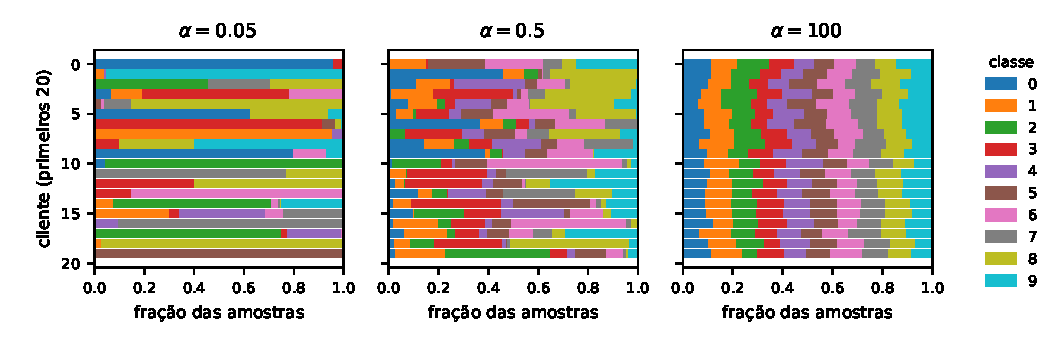
\includegraphics[width=0.92\textwidth]{figs/particoes.pdf}
    \caption{Distribuição de rótulos nos 20 primeiros dos 100 clientes para três valores de $\alpha$, em um conjunto balanceado de 10 classes com 5.000 amostras cada (como o CIFAR-10). Cada barra é um cliente, e as cores indicam a fração de cada classe. Gerada por \texttt{scripts/fig\_particoes.py} com semente 0 e mínimo de 5 amostras por cliente.}
    \label{fig:particoes}
\end{figure*}

Os algoritmos de referência (bloco B) entram em C1. Eles mostram se o ganho do FedProx, quando existe, é grande ou pequeno diante de alternativas que deslocam a correção para o servidor e não custam nada ao cliente.

\subsection{Fluxo de execução}
\label{sec:fluxo}

A Figura~\ref{fig:fluxo} resume o fluxo completo, da preparação dos dados à análise. Duas verificações antecedem a grade completa. A primeira é um \textbf{piloto} no Fashion-MNIST, com uma semente e 20 rodadas, que valida o \textit{pipeline} e mede o tempo real por execução para confirmar o orçamento. A segunda é o \textbf{teste de sanidade} entre FedProx com $\mu = 0$ e FedAvg: com a mesma semente e algoritmos determinísticos habilitados, as duas execuções devem produzir curvas de acurácia idênticas. Qualquer diferença indica falha no pareamento ou na implementação.

\begin{figure}[ht]
    \centering
    \begin{tikzpicture}[
        font=\scriptsize,
        etapa/.style={draw, rounded corners=2pt, fill=azul!6, text width=5.6cm, align=center, minimum height=0.55cm},
        dec/.style={draw, diamond, aspect=3.2, fill=gray!10, align=center, inner sep=1pt},
        arr/.style={-{Stealth[length=4pt]}, thick},
        node distance=0.3cm
    ]
        \node[etapa] (s1) {1. Preparar ambiente (Kaggle) e baixar datasets};
        \node[etapa, below=of s1] (s2) {2. Piloto: F-MNIST, 1 semente, 20 rodadas};
        \node[dec, below=of s2] (d1) {$\mu{=}0 \equiv$ FedAvg?\\ tempo ok?};
        \node[etapa, below=of d1] (s3) {3. Blocos A e B (exploratório, 5 sementes)};
        \node[etapa, below=of s3] (s4) {4. Escolher $\mu^*$ por dataset};
        \node[etapa, below=of s4] (s5) {5. Blocos C e D (tipos de desvio; 10 sementes novas)};
        \node[etapa, below=of s5] (s6) {6. Micro-experimento de custo em CPU (C4)};
        \node[etapa, below=of s6] (s7) {7. Análise: curvas, mapa $\alpha\times\mu$, Wilcoxon + Holm, TOST};
        \draw[arr] (s1) -- (s2);
        \draw[arr] (s2) -- (d1);
        \draw[arr] (d1) -- node[right]{sim} (s3);
        \draw[arr] (d1.east) -- ++(0.55,0) |- node[pos=0.25, right]{não: corrigir} (s2.east);
        \draw[arr] (s3) -- (s4);
        \draw[arr] (s4) -- (s5);
        \draw[arr] (s5) -- (s6);
        \draw[arr] (s6) -- (s7);
    \end{tikzpicture}
    \caption{Fluxo de execução experimental.}
    \label{fig:fluxo}
\end{figure}

Na etapa 7, o script de análise produz quatro artefatos: (i) curvas de acurácia por rodada, com média e desvio padrão entre sementes, para cada $\alpha$; (ii) um mapa de calor do ganho médio $\Delta$ do FedProx sobre o FedAvg, nos eixos $\alpha$ e $\mu$ (bloco A, descritivo); (iii) a tabela de $R_\tau$ e custo total até o alvo, com a fração de execuções que atinge $\tau$; e (iv) a tabela de testes estatísticos (Wilcoxon e TOST) dos blocos C e D. Esses artefatos são a base da Seção~\ref{sec:resultados}.
